\documentclass[conference,letterpaper]{IEEEtran}
% Four technical pages and a reference-only fifth page. No margin/font shrinking.
\usepackage[T1]{fontenc}
\usepackage{newtxtext,newtxmath}
\usepackage{amsmath,booktabs,array,tabularx}
\usepackage{graphicx,tikz}
\usetikzlibrary{arrows.meta,positioning,calc}
\usepackage{cite}
\usepackage[hidelinks]{hyperref}
\usepackage{microtype}
\newcommand{\epl}{EP-L2}
\newcommand{\base}{B16}
\newcommand{\unif}{U-WB16}
\newcolumntype{L}[1]{>{\raggedright\arraybackslash}p{#1}}
\hypersetup{pdftitle={EP-L2: Decoupling Tag Residency from Dirty-Data Lifetime in GPU L2 Caches},pdfauthor={EP-L2 project; author information pending},pdfsubject={EN-v7: ownership transfer, five H0 pairs and independently audited downstream sensitivity}}
\hyphenation{write-back micro-ar-chi-tec-ture in-di-rec-tion}
\begin{document}
\title{EP-L2: Decoupling Tag Residency from\\Dirty-Data Lifetime in GPU L2 Caches}
\author{\IEEEauthorblockN{Author information to be completed}\IEEEauthorblockA{English working draft EN-v7 --- not for submission}}
\maketitle
\begin{abstract}
Eviction ends tag residency before a dirty line's obligations end: data must survive until downstream acceptance, and address ordering may persist until writeback completion. A fixed-partition L2 bridges these lifetimes by copying unchanged bytes into a writeback buffer. EP-L2 instead transfers ownership: the victim retains its original banked slot, the incoming resident obtains a distinct legal landing, and local data and ordering state retire separately. At equal tag count, payload capacity, and modeled bank service, five complete non-atomic workload pairs eliminate all resident-to-writeback copies but yield only a 1.001600 geometric-mean speed ratio, including one slowdown. Under matched downstream controls, neither design records local-buffer refusals, yet U-WB's relative performance does not uniformly improve. These results distinguish reduced internal work from application progress; competitive static allocation and physical implementation cost remain unresolved.
\end{abstract}

\begin{IEEEkeywords}
GPU, L2 cache, writeback, tag--data decoupling, resource sharing
\end{IEEEkeywords}

\section{Introduction}
Eviction does not end every obligation of a cache line at once. Its tag can become reusable before its dirty bytes leave local storage; even then, same-address ordering may persist until writeback completes. Coupling storage locations to these roles turns a change of ownership into data movement.

In our fixed-partition GPU L2 reference, replacing a dirty line requires a resident-bank read and writeback-buffer (WBUF) write before the later send read. These operations move unchanged bytes. A full WBUF can also reject replacement despite free storage elsewhere. Such refusals expose a resource mismatch, but do not directly measure application delay.

Our insight is to treat eviction as an ownership transfer. The victim keeps its original payload slot while the incoming resident receives another bank-compatible landing. The difficulty is maintaining one transaction across bank refusals and intervening fills: victim identity, landing, and tag commit must agree. After commit, a real lower data carrier must take responsibility for the bytes before local storage is freed; writeback ordering retires later.

EP-L2 realizes this protocol without adding payload capacity or modeled bank ports. Earlier work retains dirty candidates in LLCs, exposes address-only candidates, or separates dirty metadata~\cite{vwq,lastwrite,dbi}. Our narrower question is ownership of the original physical payload after its resident tag is reused.

The evaluation separates internal work from execution. Five matched workloads eliminate copies and three avoid the reference's WBUF-data limit, yet average speed-ratio gain is only 0.160\%, with a CFD regression. Matched downstream controls examine when these local savings matter; stronger static partitions and physical cost remain necessary comparisons.

\section{Lifetime-Aware L2 Payload Storage}
\subsection{Fixed Physical Resources, Different Data Lifetimes}
The primary reference, \base{} (\texttt{B16\_BANKED}), partitions 1168 line-sized slots into 1024 resident, 128 bypass-return, and 16 WBUF slots. \unif{} (\texttt{U\_WB16}) permits resident and WB allocations across this physical pool. Each slot is 128 B with four 32-B sectors. Both modes provision four banks of 292 slots, at most one modeled line-sized operation per bank per physical GPU cycle, and a common 128-B copy latch outside the pool. Both also retain 128 writeback address-directory (WAD) entries and the same request-metadata limits. Sixteen is the static \emph{data} quota, not the U-WB control limit.

\begin{figure*}[t]
\centering
\begin{minipage}[t]{.49\textwidth}
\centering\small\textbf{(a) Logical organization of one L2 slice}\par\smallskip
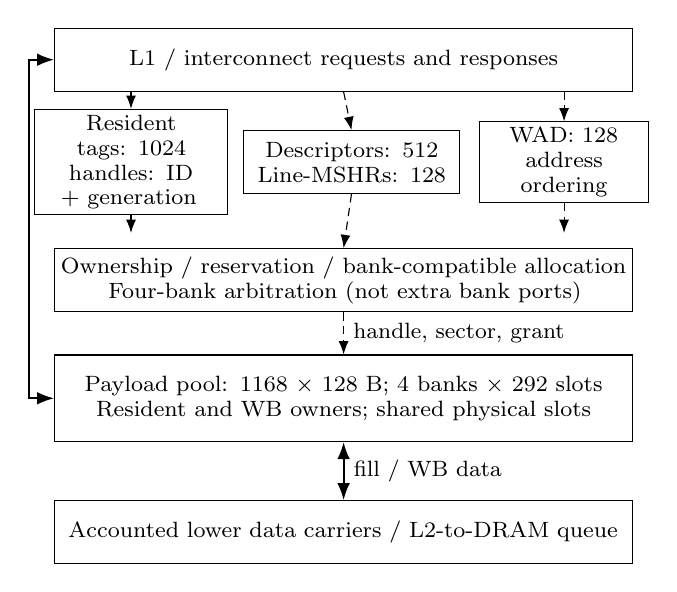
\begin{tikzpicture}[x=1mm,y=1mm,>=Latex,font=\fontsize{8}{9}\selectfont,
box/.style={draw,align=center,inner sep=2pt,minimum height=8mm},
ctl/.style={->,densely dashed,line width=.4pt},data/.style={<->,line width=.7pt}]
\node[box,text width=72mm] (in) at (40,53) {L1 / interconnect requests and responses};
\node[box,text width=23mm] (tag) at (13,40) {Resident tags: 1024\\handles: ID + generation};
\node[box,text width=26mm] (req) at (41,40) {Descriptors: 512\\Line-MSHRs: 128};
\node[box,text width=20mm] (wad) at (68,40) {WAD: 128\\address ordering};
\node[box,text width=72mm] (ctrl) at (40,25) {Ownership / reservation / bank-compatible allocation\\Four-bank arbitration (not extra bank ports)};
\node[box,text width=72mm,minimum height=11mm] (pool) at (40,10) {Payload pool: 1168 $\times$ 128 B; 4 banks $\times$ 292 slots\\Resident and WB owners; shared physical slots};
\node[box,text width=72mm] (low) at (40,-7) {Accounted lower data carriers / L2-to-DRAM queue};
\draw[ctl] (in.south)--(req.north);
\draw[ctl] (13,49)--(tag.north);\draw[ctl] (68,49)--(wad.north);
\draw[ctl] (tag.south)--(13,31);\draw[ctl] (req.south)--(ctrl.north);\draw[ctl] (wad.south)--(68,31);
\draw[ctl] (ctrl.south)--node[right]{handle, sector, grant} (pool.north);
\draw[data] (pool.south)--node[right]{fill / WB data} (low.north);
\draw[data] (in.west)--(0,53)--(0,10)--(pool.west);

\end{tikzpicture}
\end{minipage}\hfill
\begin{minipage}[t]{.49\textwidth}
\centering\small\textbf{(b) Copy removal and separate release events}\par\smallskip
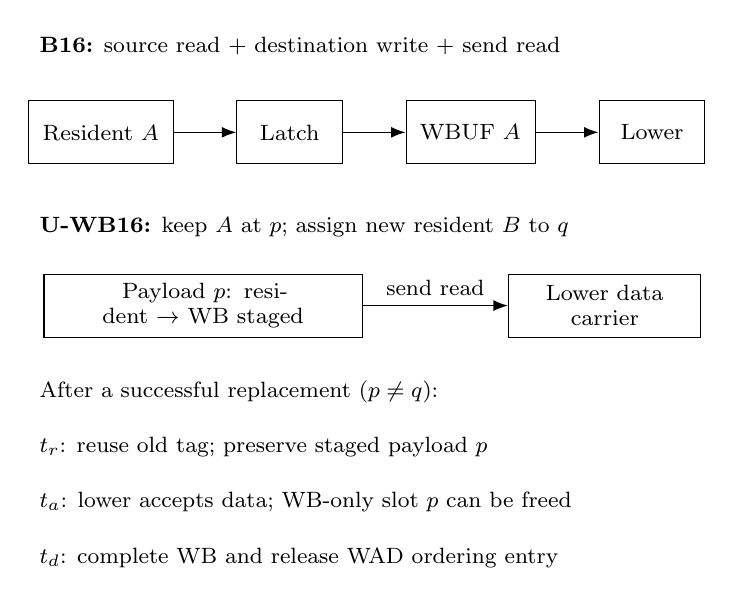
\begin{tikzpicture}[x=1mm,y=1mm,>=Latex,font=\fontsize{8}{9}\selectfont,
box/.style={draw,align=center,inner sep=2pt,minimum height=8mm},arr/.style={->,line width=.5pt}]
\node[anchor=west] at (0,55) {\textbf{B16:} source read $+$ destination write $+$ send read};
\node[box,text width=17mm] (a) at (9,44) {Resident $A$};
\node[box,text width=12mm] (l) at (33,44) {Latch};
\node[box,text width=15mm] (w) at (56,44) {WBUF $A$};
\node[box,text width=12mm] (d) at (79,44) {Lower};
\draw[arr] (a)--(l);\draw[arr] (l)--(w);\draw[arr] (w)--(d);
\node[anchor=west] at (0,32) {\textbf{U-WB16:} keep $A$ at $p$; assign new resident $B$ to $q$};
\node[box,text width=39mm] (p) at (22,22) {Payload $p$: resident $\to$ WB staged};
\node[box,text width=23mm] (lo) at (73,22) {Lower data carrier};
\draw[arr] (p)--node[above]{send read} (lo);
\node[anchor=west] at (0,11) {After a successful replacement ($p\ne q$):};
\node[anchor=west] at (0,4) {$t_r$: reuse old tag; preserve staged payload $p$};
\node[anchor=west] at (0,-3) {$t_a$: lower accepts data; WB-only slot $p$ can be freed};
\node[anchor=west] at (0,-10) {$t_d$: complete WB and release WAD ordering entry};
\end{tikzpicture}
\end{minipage}
\caption{From relocation to ownership transfer. (a) Resident tags, requester descriptors, and writeback address ordering are separately tracked around a fixed banked payload pool. (b) B16 copies an evicted dirty line to its WBUF; U-WB retains the bytes at $p$ while allocating a different landing $q$ for the incoming resident. Local storage is released after lower data acceptance, whereas address ordering persists to writeback completion. Both modes have equal data capacity, bank service, and a common copy latch. TVD/RO and concurrent dynamic bypass are outside the reported WB-only evaluation.}
\label{fig:organization}
\end{figure*}


Figure~\ref{fig:organization} shows the declared service model. WB-only pooling can borrow reference bypass-return slots, but concurrent dynamic bypass use is unvalidated. Idle bypass capacity therefore makes a WB-heavy static control important.

A resident tag names a payload through a slot identifier and generation. Each slot has one authoritative owner; ready/pending sector masks and pins track its consumers. The initial design preserves the resident bank class:
\begin{equation}
 \operatorname{bank}(p)=p\bmod4=\operatorname{tag\_index}\bmod4.
\label{eq:bank}
\end{equation}
A globally free slot is therefore not necessarily a legal landing for a given tag. The 1024 tags bound resident visibility; a temporarily reserved incoming landing is not an additional visible resident line.

\subsection{Eviction as an Ownership Transfer}
For dirty victim $A$ in slot $p$, B16 reads the resident and writes WBUF before the send read. U-WB16 changes $p$'s owner to \texttt{WB\_STAGED} and reserves distinct $q\ne p$ for incoming $B$. The landing must match the tag's bank class. Two copy operations disappear; send read and lower data carriage remain.

The serialized frontend first checks issue-queue/MSHR needs, victim pins and pending sectors, WAD capacity, and legal staging/landing availability. Its pending transaction records requester, victim tag index, old payload handle, and acquired resources. A later probe by the same request uses this held victim, even if another way's fill changes the raw LRU candidate. A different frontend request is refused while this transaction is pending. Bank denial retains its identity and reservations for retry.

In B16, a common latch bridges the victim read and staging write. In U-WB16, the reserved incoming landing remains separate from the old dirty slot. Any incoming write obtains its bank grant before ownership is changed. The controller provisionally installs the landing, then invokes underlying tag access; refusal rolls back uncommitted reservations and restores the saved victim/tag identity. Consumed bank operations remain charged. Successful underlying access binds the dirty writeback and clears the pending transaction. Directed tests exercise intervening fills and cross-cycle victim identity.

\subsection{Progress and Independent Retirement}
At successful replacement $t_r$, the old tag becomes reusable while $p$ remains protected (Fig.~\ref{fig:organization}). After a granted send read and actual lower-FIFO push at $t_a$, the packet carries the dirty data and local $p$ is released. WAD address ordering remains until writeback completion $t_d$. A late event follows its own handle/transaction identity, not the reused tag.

Requester descriptors and pins survive until response acceptance or internal consumption. Generation identity and per-sector readiness prevent a ready sector from implying a ready line. Eventual lower service and stable bank retry identity are necessary for local progress; whole-GPU deadlock freedom is not established.

\begin{figure*}[t]
\centering
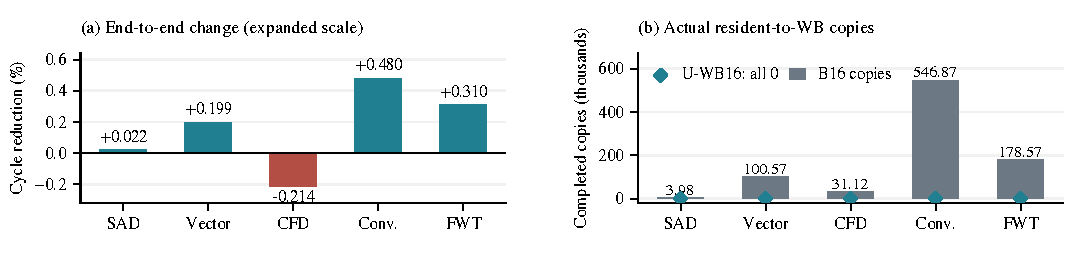
\includegraphics[width=\textwidth]{figures/fig2_results.pdf}
\caption{Five H0 workload pairs; sensitivity results are reported separately. (a) Cycle reduction $100(C_B-C_U)/C_B$, on an expanded scale with zero denoting B16; CFD regression is retained. The speed-ratio geomean is 1.001600, not the mean of these percentages. (b) Actual completed 128-B copies; U-WB16 is zero in every pair. Vector, Conv., and FWT denote vectorAdd\_4M, convolutionSeparable, and FWT\_7\_21. No error bars or significance claim.}
\label{fig:mainresults}
\end{figure*}

\subsection{Implementation Cost and Extension Boundary}
The pool holds 146 KiB/slice, or 9.125 MiB across 64 slices; common 128-B latches add 8 KiB/chip. An 11-bit index identifies a slot. Tags need $1024(11+G)$ handle bits for generation width $G$, and up to 128 WB handles need $128(11+G)$ bits plus control state. These gross representations are not incremental area: the reference already has common fields.

Added control includes bank-compatible allocation, handle/owner checks, pins, and rollback. Concrete SRAM ports, generation bounds, pipelines, and lower data carriers require implementation. Equal modeled capacity/service does not establish equal hit latency, timing, area, or energy; no RTL synthesis, STA, or power measurement is available. TVD and oracle-based RO are disabled, and neither has qualified application results here; Ideal diagnostics are also outside this evaluation.

\section{Experimental Methodology}
\subsection{Matched Resources and Complete Inputs}
We use the Accel-Sim SASS flow and GPGPU-Sim performance-model lineage~\cite{accelsim,gpgpusim}. Their published validation does not validate this modified L2. B16 and U-WB16 execute with the same independently qualified binary, complete trace input, non-mode settings, timing scope, and termination rules. Table~\ref{tab:configuration} records the modeled configuration, including the modified L2; it is not a reconstruction of undocumented commercial-cache internals.

\begin{table}[t]
\caption{Declared matched configuration. L2 capacities are per slice.}
\label{tab:configuration}\centering\footnotesize
\begin{tabularx}{\columnwidth}{@{}L{.42\columnwidth}X@{}}
\toprule
Resource & Setting \\
\midrule
Compute / clock domains & 80 SMs; core/ICNT/L2: 1132 MHz; DRAM: 850 MHz \\
L1 (fixed) & 64 KiB/SM; 4 banks; 20-cycle setting \\
L2 tags / data & 1024 tags; 1168 slots, 146 KiB \\
Line / sectors / banks & 128 B / $4\times32$ B / $4\times292$ slots \\
Service / common latch & 1 op/bank/physical cycle / 128 B \\
Descriptors / Line-MSHRs & 512 / 128; 32 requesters/address \\
WAD / lower queue & 128 / 128 entries \\
Chip / memory channels & 64 slices / 32 channels \\
L2 ROP delay & 160-cycle model setting \\
DRAM scheduler / return & 128 / 192 entries per channel \\
\bottomrule
\end{tabularx}
\end{table}

The fixed development set is convolutionSeparable, FWT\_7\_21, cfd\_097k, vectorAdd\_4M, and SAD. Artifacts bind each complete commandlist, input size, and trace body. SAD is the predeclared negative control. All five pairs, including slowdowns, enter the geometric mean. This development set does not establish holdout or general GPU coverage.

\subsection{Validation Boundary}
Independent tests cover pending-victim identity, physical-cycle bank grants, host prefill, symbolic 32-B sector versions, response backpressure, and separate WB acceptance/completion. Every run closes all 64 slices' outstanding requests and resource trackers. Complete opcode auditing restricts application qualification to non-atomic inputs. SASS lacks full numerical payloads, so these checks establish transaction/lifecycle consistency rather than numerical output correctness. Reproducibility artifacts bind source, executable, ordered configurations, full commandlists/trace bodies and raw logs; all reported pairs undergo independent input, log, and terminal validation.

\section{From Saved Internal Work to Application Effects}
\subsection{Copy Removal Is Not a Speedup Model}
All five predeclared H0 workload pairs have complete trace-driven simulation results and pass the stated transaction-lifecycle checks. Each pair has equal instruction counts and matched full input/termination scope. Figure~\ref{fig:mainresults}(a) reports the complete set: SAD is almost tied; Vector, Convolution, and FWT reduce cycles by 0.199\%, 0.480\%, and 0.310\%, while CFD increases cycles by 0.214\%. The geometric mean of $C_B/C_U$ is 1.001600, or a 0.160\% speed-ratio gain. These deterministic paired observations establish neither statistical significance nor general GPU speedup.

Figure~\ref{fig:mainresults}(b) shows removal of every measured resident-to-WB copy. A committed non-rolled-back B16 writeback uses two copy operations and one send read; U-WB16 retains the send read. This local operation saving is not a speedup model. Actual WB counts also change: CFD completes 31,123/31,063 WBs and FWT 178,569/178,585 for B16/U-WB16. Consequently, the run-level logical-operation difference need not equal twice either mode's WB count.

\begin{figure*}[t]
\centering
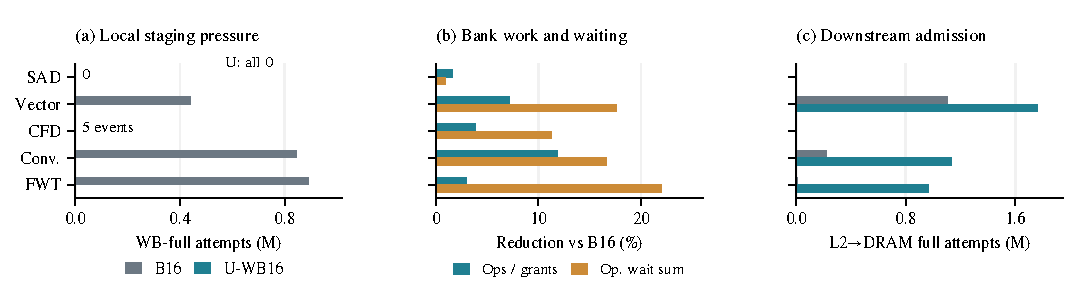
\includegraphics[width=\textwidth]{figures/fig3_pressure.pdf}
\caption{H0 application-cumulative pressure and service observations. (a) WB-data-full refusal attempts; CFD's small B16 count is labeled explicitly. (b) Separate relative reductions in logical work/successful modeled bank grants and in summed per-operation conflict waits. Logical operations and grants coincide at drain in these runs, but are independently checked counters. (c) Frontend attempts denied when the L2-to-DRAM queue is full. M denotes $10^6$. Attempt counts and operation-wait sums are not elapsed GPU cycles or unique transactions; reductions and increases do not establish causality.}
\label{fig:causal}
\end{figure*}

\subsection{Local Staging Relief and Its Downstream Cost}
Vector, Convolution, and FWT record 440,161, 845,097, and 890,294 B16 WB-data-full events; U-WB16 records zero. Figure~\ref{fig:causal}(b) shows less modeled bank work and lower aggregate conflict waits. Successful grants are actual model-service observations, not estimates obtained by multiplying copies. At drained termination, their equality to logical operations implies neither elapsed-time nor RTL timing/energy savings.

For the same three workloads, L2-to-DRAM full-block attempts rise from 1.104M to 1.764M, 0.218M to 1.132M, and 0.013M to 0.968M. This is consistent with pressure moving downstream after local staging relief. It does not independently identify the limiting queue or DRAM service. Denials may repeat for one frontend head and overlap other blockers. From final cumulative observations of all 32 channels, the modeled issued-byte/atom-cycle fractions are 64.5/64.8\% for Convolution and 14.1/14.1\% for FWT. Even frequent queue denials therefore do not prove global DRAM-bandwidth saturation. Kernel-boundary cumulative snapshots are not summed.

CFD is a useful counterexample: despite removing copies and lowering bank waits from 102,546 to 91,029, U-WB16 takes 169 more cycles. WAD-hazard events increase from 9,841 to 13,400, WB counts differ, and successful DRAM writes change from 3,983,744 to 3,976,064~B. These correlated changes motivate ordering/service diagnosis; they do not identify a unique cause. SAD has no observed WB-data-full pressure and differs by only 24 cycles. Neither case is discarded.



\subsection{Separating Buffer Headroom from Service Speed}
Q4 expands downstream queues, scheduler/return storage and credits; D4 retains Q4 buffering and raises the DRAM domain (Table~\ref{tab:headroom}). Both compare B16/U-WB under identical conditions without changing L2 capacity/service. Buffers affect scheduling visibility and cost~\cite{sms}; D4 shortens physical DRAM timing while preserving the fixed 100-GPU-cycle interface delay. Neither intervention is free hardware or pure bandwidth.

\begin{table}[t]
\caption{Matched downstream sensitivity settings; core/ICNT/L2 remain 1132\,MHz.}
\label{tab:headroom}\centering\footnotesize
\begin{tabular}{@{}lrrr@{}}
\toprule
Resource & H0 & Q4 & D4 \\
\midrule
L2$\to$DRAM / DRAM$\to$L2 & 128/64 & 512/256 & 512/256 \\
Scheduler / return queues & 128/192 & 512/768 & 512/768 \\
Derived shared credits & 319 & 1279 & 1279 \\
DRAM clock (MHz) & 850 & 850 & 3400 \\
\bottomrule
\end{tabular}
\end{table}

For condition $h$, define $S_w(h)=C_{B,w}(h)/C_{U,w}(h)$ and $J_w(h)=S_w(h)/S_w(\mathrm{H0})$. All four cycles are retained; speeding both modes does not itself improve U-WB's relative effect. Diagnostic means never enter the five-workload H0 mean.

\begin{table}[t]
\caption{Paired cycles under matched service conditions. $S=C_B/C_U$; $J=S/S(\mathrm{H0})$. Q4 observations here cover Convolution only.}
\label{tab:downstreamresults}\centering\footnotesize
\begin{tabular}{@{}lrrrr@{}}
\toprule
Workload, $h$ & $C_B$ & $C_U$ & $S$ & $J$ \\
\midrule
Conv., H0 & 292,932 & 291,525 & 1.004826 & 1.000000 \\
Conv., D4 & 267,521 & 268,544 & 0.996191 & 0.991406 \\
Conv., Q4 & 290,333 & 293,709 & 0.988506 & 0.983758 \\
FWT, H0 & 493,189 & 491,662 & 1.003106 & 1.000000 \\
FWT, D4 & 452,758 & 451,254 & 1.003333 & 1.000226 \\
\bottomrule
\end{tabular}
\end{table}

D4 accelerates both modes relative to H0 (Table~\ref{tab:downstreamresults}), but Convolution reverses U-WB's advantage: it takes 1023 more cycles than B16. FWT saves 1504 cycles, close to its H0 saving of 1527. The two-workload D4 geometric mean is 0.999755$\times$, with interaction 0.995806$\times$; this diagnostic result does not replace the five-workload H0 mean. More downstream headroom does not uniformly amplify the mechanism's benefit.

D4 records no WB-data-full, L2-to-DRAM-full, or scheduler-full attempts in either mode, yet modeled bank-wait sums rise relative to H0. Observed zeros do not establish globally nonbinding service. Q4 Convolution also removes WBUF/lower-queue-full attempts, but U-WB is 3376 cycles slower; WAD-full attempts are 55,645/54,516 for B16/U-WB. Local data can leave well before ordering obligations retire. These repeated event counts identify candidate constraints, not unique stalls or a proven critical path. Staging durations start at B16's copy readout versus U-WB's producer commit, so only same-mode, across-condition comparisons share endpoints. Further attribution requires matched service and ordering evidence.


An equal-total strong static repartition remains unevaluated. Thus, current results combine copy removal and pooling; they do not isolate dynamic elasticity from a better fixed WB quota. Static allocation, service regime, and implementation cost bound the present performance claim.

\section{Relation to Prior Storage Decoupling}
VWQ exposes dirty LLC candidates to scheduling while retaining a physical write queue~\cite{vwq}. Decoupled last-write prediction tracks candidate addresses separately while data remain in LLC; evicted dirty blocks use another write buffer~\cite{lastwrite}. DBI groups dirty metadata outside tags by DRAM row~\cite{dbi}. EP-L2 instead tracks the original slot after tag reuse, its distinct incoming landing, and separate payload/order retirement. DBI dirtiness is not WAD's in-flight address ordering.

V-Way separates tag/data placement~\cite{vway}; Tag-Split Cache changes storage granularity~\cite{tsc}. Unified GPU memory shares SM-local register/cache/scratchpad storage~\cite{unified}. In-cache MSHRs~\cite{farkas}, MiCache's shared FPGA data/MSHR storage~\cite{micache}, and DL-MSHR's linked slots that also hold write-miss data~\cite{dlmshr} concern different shared resources. Our comparison fixes resident-tag and miss-tracking budgets.

\section{Conclusion}
Eviction need not relocate dirty data when a tag becomes reusable. EP-L2 preserves the victim's slot, allocates a legal incoming landing, and retires payload storage separately from writeback ordering. Five complete workloads eliminate copies but yield only a 1.001600 geometric-mean speed ratio. Reduced bank work and staging pressure therefore do not guarantee faster execution. Matched downstream controls do not uniformly amplify U-WB's relative benefit. Competitive static allocation and physical cost remain unresolved.

% The fifth page contains references only.
\clearpage
\bibliographystyle{IEEEtran}
\bibliography{references_verified}
\end{document}
